\documentclass[aps,prb,onecolumn,notitlepage,showpacs,floatfix,superscriptaddress]{revtex4-1}
\usepackage{dcolumn}
\usepackage{tabularx}
\usepackage{bm}
\usepackage{soul}
\usepackage{amsmath,amssymb,graphicx}
\usepackage[colorlinks=true,citecolor=blue,urlcolor=blue,linkcolor=blue]{hyperref}
\usepackage{environ}

\NewEnviron{eqnsplit}{%
\begin{equation}
\begin{split}
  \BODY
\end{split}
\end{equation}
}

\newcommand{\mrm}[1]{\mathrm{#1}}
\newcommand{\ang}{\mathrm{\AA}}

\bibliographystyle{apsrev4-1}

%%%%%%%%%%%%%%%%%%%%%%%%%%%%%%%%%%%%%%%%%%%%%%%%
\begin{document}
\title{Scattering Theory}

\author{Avinash Rustagi}
\email{arustag@ncsu.edu}
\affiliation{Department of Physics, North Carolina State University, Raleigh, NC 27695}
%
\date{\today}
%%%%%%%%%%%%%%%%%%%%%%%%%%%%%%%%%%%%%%%%%%%%%%%%

\maketitle
Scattering is one of the most important experimental probes that are particularly useful in characterizing a system. X-ray and electron scattering provides information about the lattice, neutron scattering provides information about the magnetic properties. Rutherford postulated the atoms being composed of a point like nucleus through scattering experiment.
\begin{figure}[hbtp]
\centering
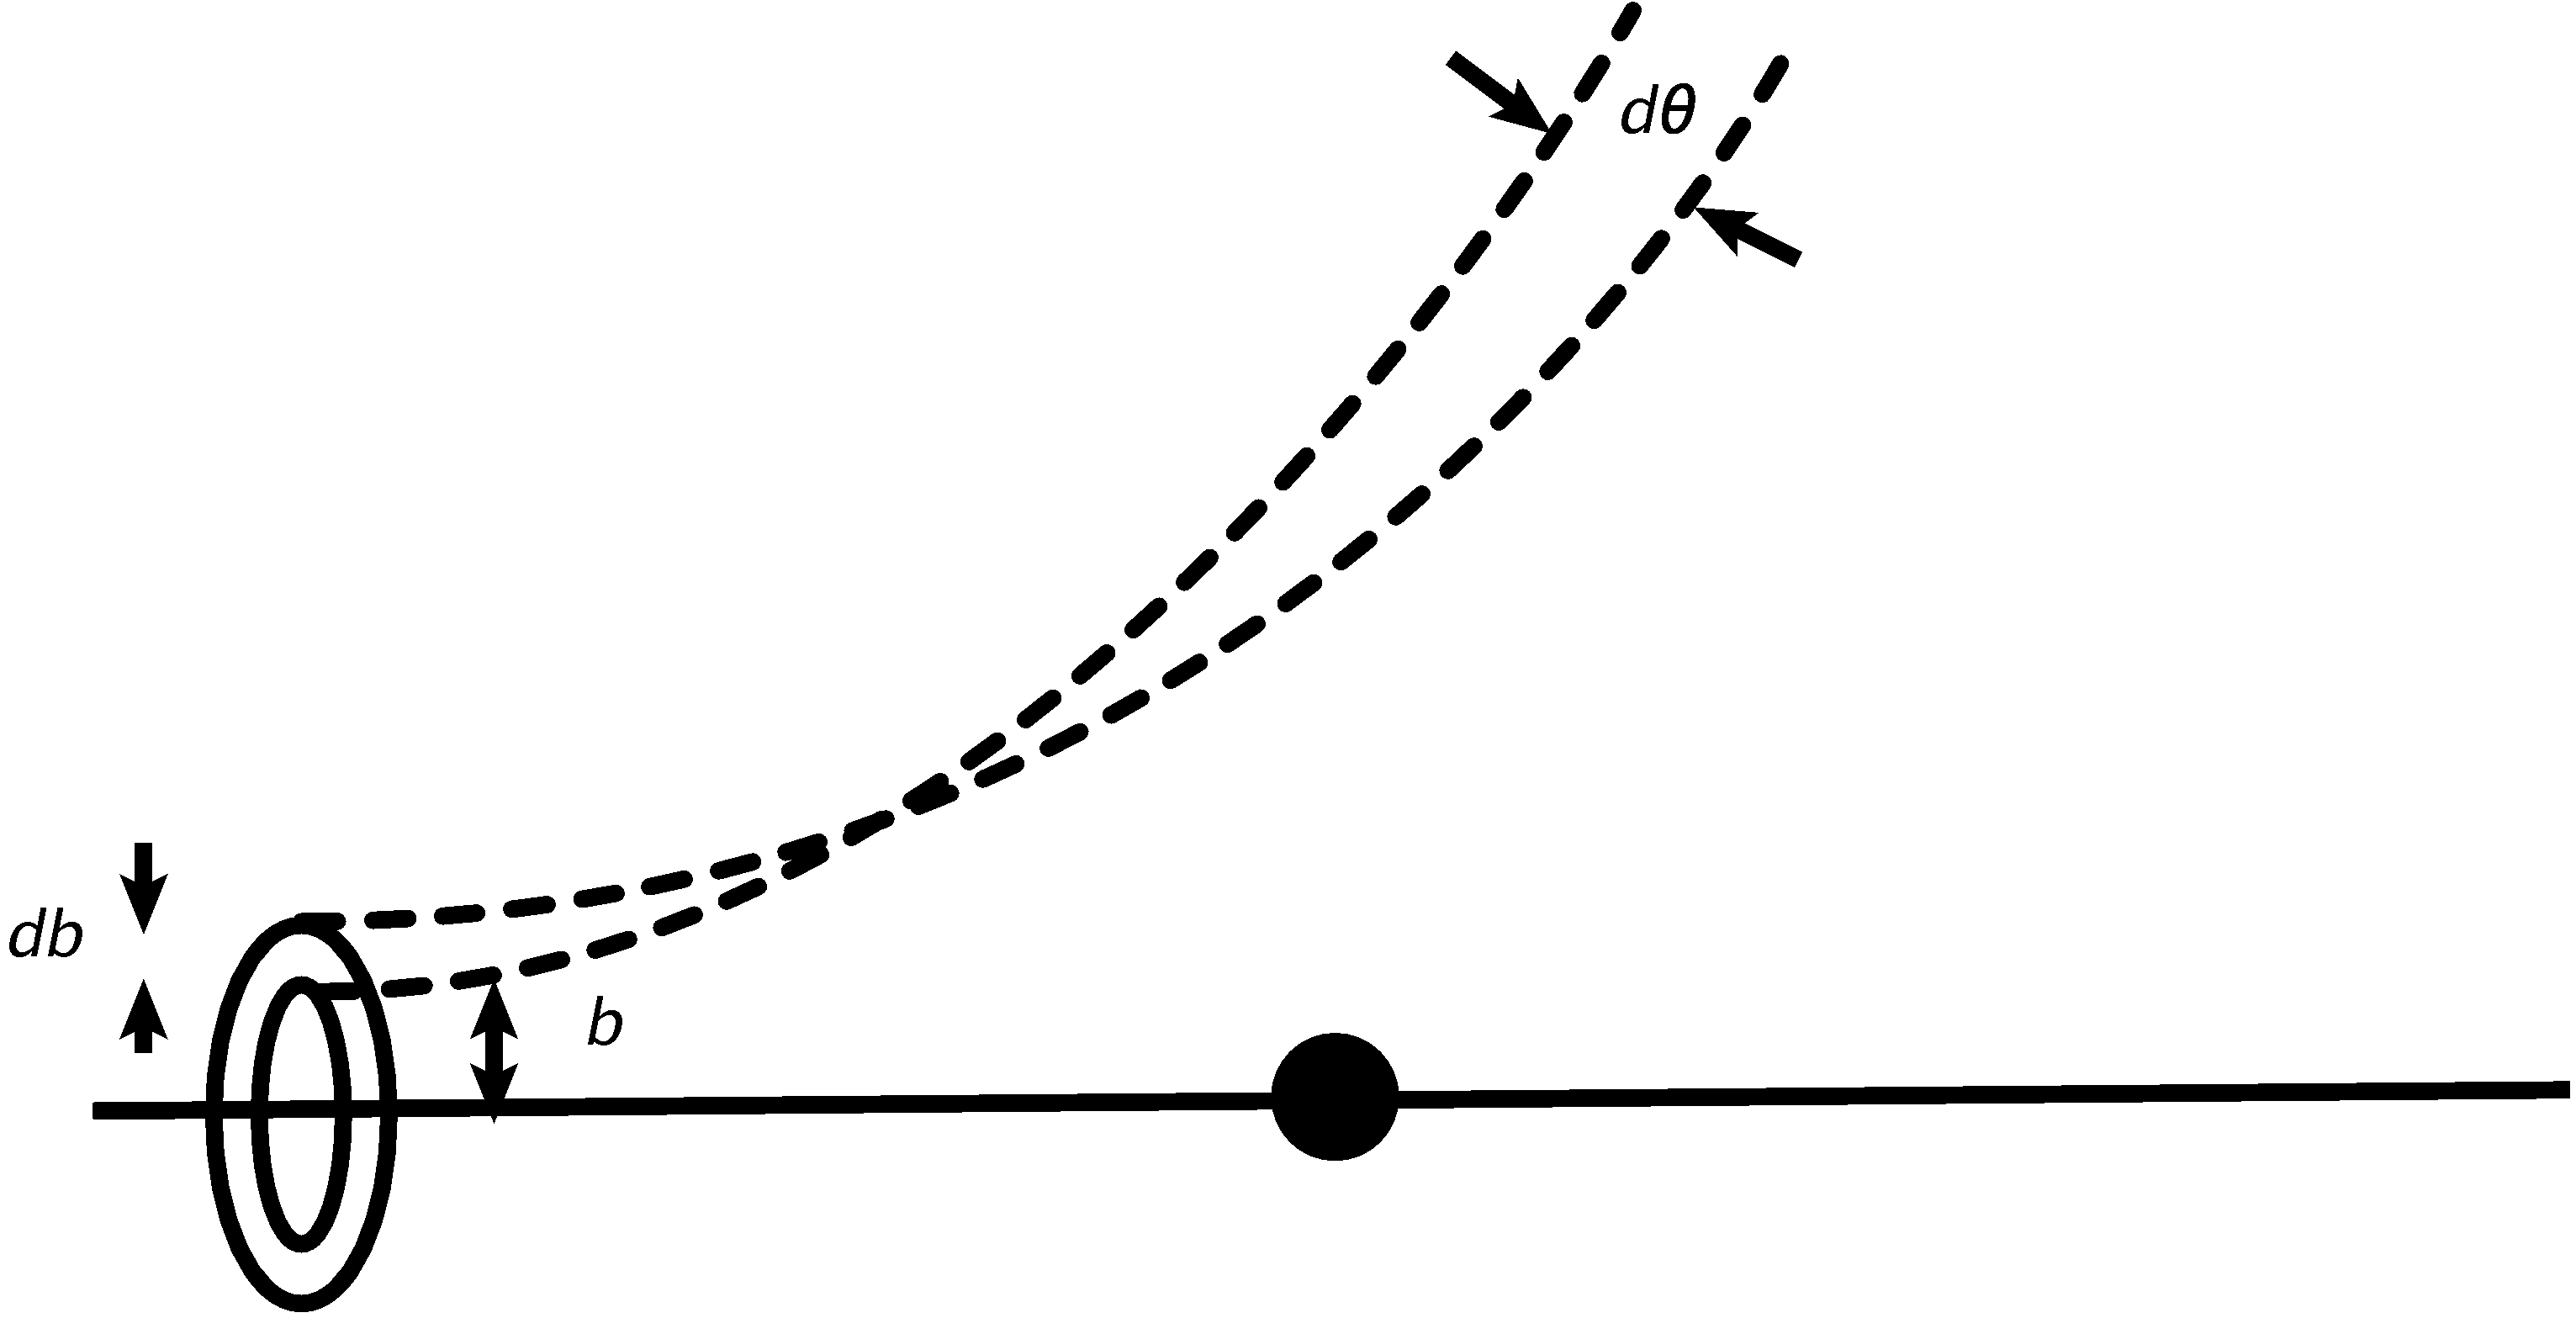
\includegraphics[scale=0.1]{Cross_Section.png}
\caption{Scattering cross-section schematic.}
\end{figure}

Scattering is when an incident flux of particles interact with some potential and are deflected. The information about the scattering potential is encoded in the scattering cross-section. The differential scattering cross-section $\sigma(\theta,\phi)$ is the ratio of scattered flux to the incident flux i.e. the number of scattered particles per unit incident flux in a solid angle $d\Omega$. Assuming azimuthal symmetry, for an incident flux of particles $J_I$, the number of particles scattered in solid angle $[\Omega,\Omega+d\Omega]$ is
\begin{equation}
dn = J_I \sigma(\theta,\phi) d\Omega = J_I \sigma(\theta,\phi)\sin\theta d\theta d\phi
\end{equation}
This is related to the impact factor/distance when the particles are far away from the scattering potential
 \begin{equation}
dn = J_I bdbd\phi
\end{equation}
Thus we can read off the expression for differential scattering cross-section $\sigma(\theta,\phi)$
\begin{equation}
\sigma(\theta,\phi) = \dfrac{b}{\sin\theta} \dfrac{db}{d\theta}
\end{equation}

\section{Rutherford Scattering}
\begin{figure}[hbtp]
\centering
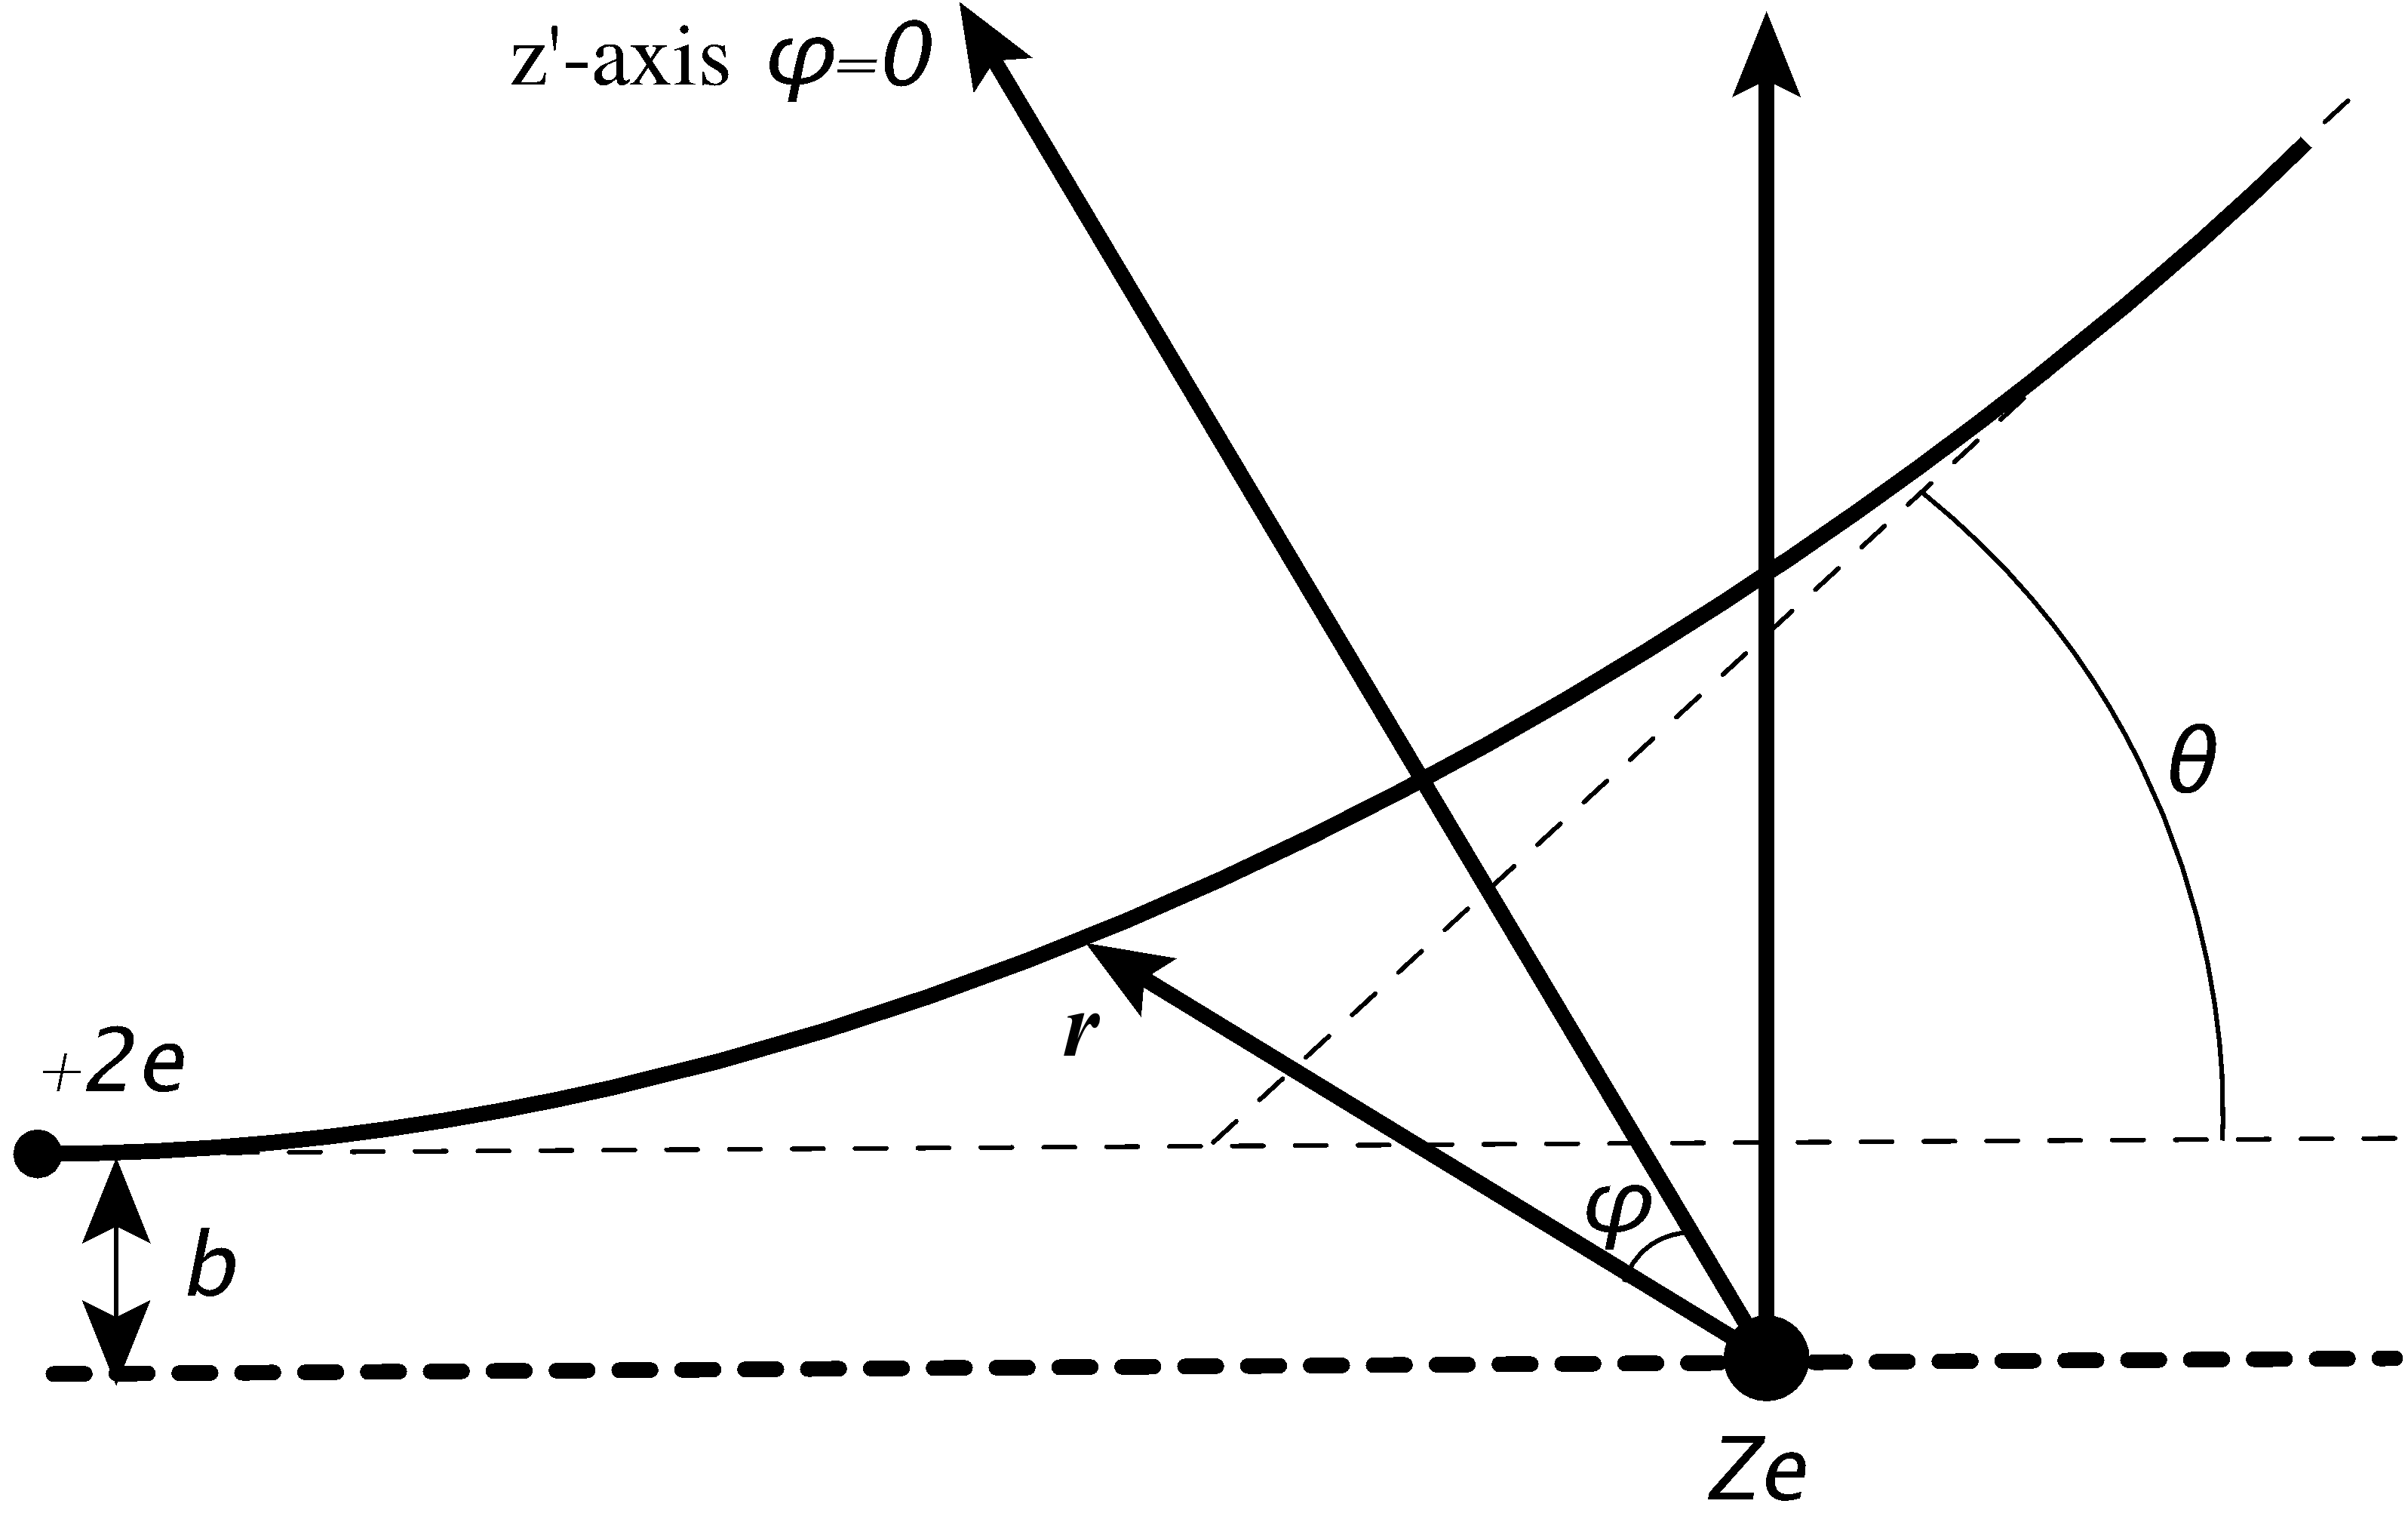
\includegraphics[scale=0.1]{Rutherford.png}
\caption{Rutherford Scattering cross-section schematic.}
\end{figure}
Rutherford scattering is the scattering of a light charged particle from a heavy charged nucleus. The scattering potential is Coulomb
\begin{equation}
V(r)=\dfrac{\kappa}{r}
\end{equation}
where ${\bm r}$ is the vector connecting the particle and the nucleus. The force is therefore
\begin{equation}
{\bm F} = \dfrac{\kappa}{r^2	} \dfrac{{\bm r}}{r}
\end{equation}
As shown in the scattering schematic, the particle deflection is symmetric about the z'-axis ($\phi=0$). Note that $\phi$ is not the azimuthal angle but just a variable. Given the force, we can compute the change in momentum along the z'-axis.
\begin{equation}
{\bm F}=\dfrac{d{\bm p}}{dt} \Rightarrow \Delta p_{z'} = \int F_{z'} dt 
\end{equation}
Let us consider, the instant when the particle is at a distance $r$ from the scattering center shown in schematic at an angle $\phi$ from the z'-axis. 
\begin{equation}
\Delta p_{z'} = \int F_{z'} dt = \int F \cos\phi \, dt = \int \dfrac{\kappa}{r^2} \cos\phi \, dt
\end{equation}
To evaluate this integral, what comes to rescue is the conservation of angular momentum since Coulomb interaction is a central potential (acts along the radial vector) and thus has no torque. When the particle is far away from the scattering potential at a impact distance $b$ and velocity $v_0$, the angular momentum is
\begin{equation}
L=mv_0 b
\end{equation}
Now when the particle is at distance $r$ from the nucleus, 
\begin{equation}
{\bm L} = {\bm r} \times {\bm p} =m {\bm r} \times {\bm v} = m {\bm r} \times \left[ \dfrac{dr}{dt} \hat{r} + r \dfrac{d\phi}{dt} \hat{\phi} \right] = m r^2 \dfrac{d\phi}{dt} (\hat{r}\times\hat{\phi})
\end{equation}
Thus conservation of angular momentum implies
\begin{equation}
mv_0 b = mr^2 \dfrac{d\phi}{dt} \Rightarrow dt = \dfrac{r^2}{v_0 b} d\phi
\end{equation}
Therefore
\begin{equation}
\Delta p_{z'} =  \int \dfrac{\kappa}{r^2} \cos\phi \, dt = \int \dfrac{\kappa}{r^2} \cos\phi \,  \dfrac{r^2}{v_0 b} d\phi = \dfrac{\kappa}{v_0 b} \int\cos\phi \, d\phi
\end{equation}
The angular variable $\phi$ changes from $\phi_<$ to $\phi_>$, thus the total change in z'-component of momenta is
\begin{equation}
\Delta p_{z'} = \dfrac{\kappa}{v_0 b} \int_{\phi_<}^{\phi_>}\cos\phi \, d\phi = \dfrac{\kappa}{v_0 b} [\sin\phi_{>}-\sin\phi_{<}]
\end{equation}
Given the trajectory being symmetric about the z'-axis, $\phi_> = -\phi_<$ and $\phi_{>}+\vert \phi_< \vert +\theta =\pi$ 
\begin{equation}
\phi_> = \dfrac{1}{2}(\pi-\theta) \qquad \phi_< = -\dfrac{1}{2}(\pi-\theta)
\end{equation}
Therefore
\begin{equation}
\Delta p_{z'} = \dfrac{2\kappa}{v_0 b} \sin\phi_{>} =  \dfrac{2\kappa}{v_0 b} \sin\left(\dfrac{\pi}{2}-\dfrac{\theta}{2} \right)= \dfrac{2\kappa}{v_0 b} \cos\left(\dfrac{\theta}{2} \right)
\end{equation}
Assuming that the nucleus is heavy and thus the scattering of the incident particle does not change its energy whatsoever, the initial and final energy of the scattered particle are equal which means that the magnitude of momentum stays constant. 
\begin{equation}
\vert {\bm p}_f \vert = \vert {\bm p}_i \vert = p = m v_0
\end{equation}
\begin{figure}[hbtp]
\centering
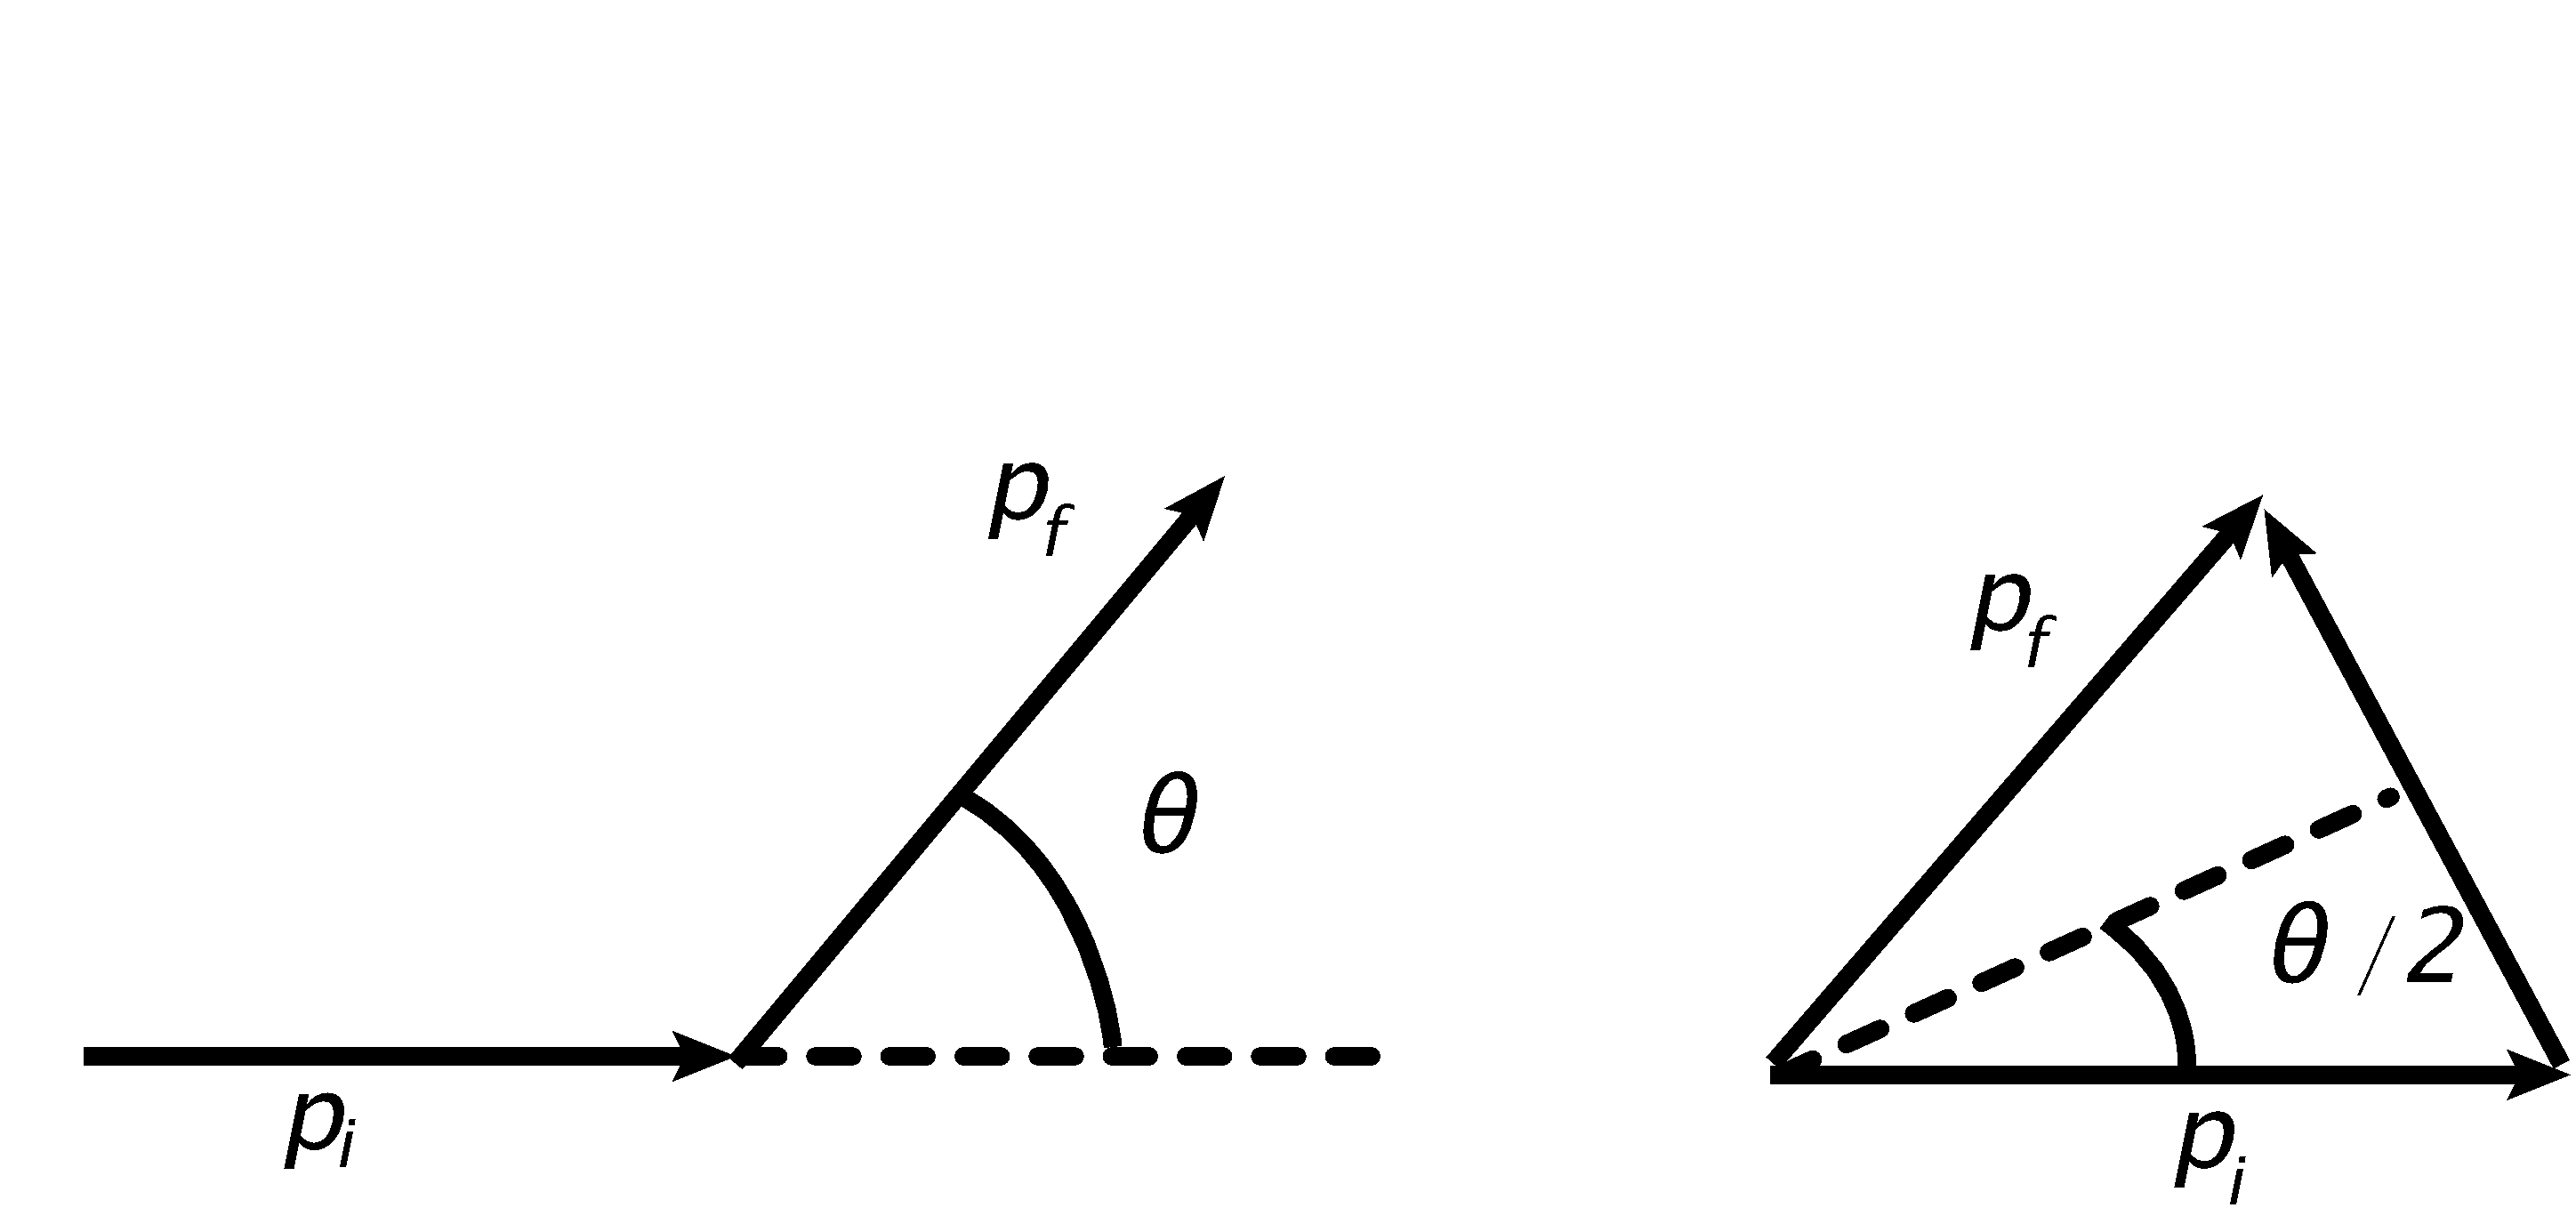
\includegraphics[scale=0.1]{momentum.png}
\caption{Momentum relation.}
\end{figure}
\begin{equation}
\Delta p_{z'} = \vert{\bm p}_f -{\bm p}_i \vert = 2 p \sin(\theta/2)
\end{equation}
Therefore
\begin{equation}
 2 p \sin(\theta/2) =  \dfrac{2\kappa}{v_0 b} \cos(\theta/2) \Rightarrow b = \dfrac{\kappa}{v_0 p} \cot(\theta/2)
\end{equation}
Thus the Rutherford scattering cross section is
\begin{equation}
\sigma(\theta) = \dfrac{b}{\sin\theta} \dfrac{db}{d\theta} =  \dfrac{\cot(\theta/2)}{\sin\theta}  \left(\dfrac{\kappa}{v_0 p}\right)^2 \dfrac{1}{2\sin^2(\theta/2)} = \left(\dfrac{\kappa}{2 v_0 p}\right)^2 \dfrac{1}{\sin^4(\theta/2)} = \dfrac{\kappa^2}{16 E^2} \dfrac{1}{\sin^4(\theta/2)}
\end{equation}

\section{Partial Wave Analysis}
Let us consider the quantum mechanical treatment of the scattering phenomenon. If we consider that all incident particles are represented by wavepackets, then the objective is to solve the Schrodinger equation for such a wavepacket
\begin{equation}
i\hbar \partial_t \Psi({\bm r},t) = \left[-\dfrac{\hbar^2}{2m} \nabla^2 + V({\bm r}) \right] \Psi({\bm r},t)
\end{equation}
and subsequently determine the probability amplitude of scattered waves in a particular direction. If the particles are incident for long times compared to the scattering time scale, then we can define a steady state situation. The wavepacket characterized by a specific energy will then satisfy the time-independent Schrodinger equation
\begin{equation}
E  \Psi({\bm r}) = \left[-\dfrac{\hbar^2}{2m} \nabla^2 + V({\bm r}) \right] \Psi({\bm r})
\end{equation}
subject to the condition that the incoming wavepacket component has the wavefunction of a plane wave $e^{i {\bm k}\cdot {\bm r}}=e^{ikz}$ i.e. $\bm k$ is along the z-axis. The general solution of the wavefunction far from the scattering potential region ($r \rightarrow \infty$) will be a superposition of the incident wavefunction and the scattered wavefunction
\begin{equation}
\Psi({\bm r}) \approx e^{i {\bm k}\cdot {\bm r}} + f(\theta,\phi) \dfrac{e^{ikr}}{r}
\end{equation}
The corresponding asymptotic flux is
\begin{equation}
\begin{split}
{\bm j} &= -i \dfrac{\hbar}{2m} \left[\Psi^* {\bm \nabla} \Psi - {\bm \nabla} \Psi^* \Psi \right] \\
&=\dfrac{\hbar}{m} {\bm k} + \dfrac{\hbar}{m} k \hat{r} \dfrac{\vert f(\theta,\phi)\vert^2}{r^2} + \mathcal{O}(1/r^3)
\end{split}
\end{equation}
The first terms corresponds to the incident flux whereas the next term is the scattered radial flux, thus the number of particles scattered across an area element $dA$ subtending a solid angle $d\Omega$ is
\begin{equation}
{\bm j}  \cdot \hat{r} dA = \dfrac{\hbar}{m} k  \dfrac{\vert f(\theta,\phi)\vert^2}{r^2}  r^2 d\Omega = \dfrac{\hbar}{m} k  \vert f(\theta,\phi)\vert^2 d\Omega
\end{equation}
The differential scattering cross section i.e. the ratio of scattered to the incident flux is threfore
\begin{equation}
d\sigma = \dfrac{m}{\hbar k} {\bm j}  \cdot \hat{r} dA  = \vert f(\theta,\phi)\vert^2 d\Omega
\end{equation}
The incoming plane wave can be expanded in terms of the spherical Bessel function
\begin{equation}
e^{ikz} = e^{ikr \cos\theta} = \sum_{l=0}^\infty i^l (2 l +1) j_l (k r) P_l (\cos \theta)
\end{equation}
where in the asymptotic limit ($r \rightarrow \infty$)
\begin{equation}
j_l (k r) \rightarrow \dfrac{1}{2ikr} [e^{i(kr - l\pi/2)}-e^{-i(kr - l\pi/2)}] = \dfrac{\sin(kr-l\pi/2)}{kr}
\end{equation}
Now let us consider the spherically symmetric scattering potential i.e. $V({\bm r}) = V(r)$, which means that the general solution to the Schrodinger equation is 
\begin{equation}
\Psi(r,\theta) = \sum_{l=0}^\infty R_l(r) P_l (\cos\theta) = = \sum_{l=0}^\infty \dfrac{u_l(r)}{r} P_l (\cos\theta)
\end{equation}
Thus the radial part of the Schrodinger equation is
\begin{equation}
\dfrac{d^2 u_l(r)}{dr^2} - \dfrac{l(l+1)}{r^2} u_l(r) +\dfrac{2m}{\hbar^2} [E-V(r)] u_l(r) =0
\end{equation}
If we look at the limit of $r \rightarrow \infty$, where the potential $V(r) \rightarrow 0 $, we should recover the description of a free particle. This means the solution of the general equation in the large distance limit should be similar to the $j_l(r)$ limit but in principle can have a phase shift,
\begin{equation}
R_l (k r) \rightarrow  \dfrac{\sin(kr-l\pi/2+\delta_l)}{kr}
\end{equation}
where $\delta_l$ are the phase shifts. Now comparing the wavefunctions
\begin{equation}
\begin{split}
&\sum_{l=0}^\infty a_l \dfrac{\sin(kr-l\pi/2+\delta_l)}{kr} P_l(\cos\theta) =  \sum_{l=0}^\infty i^l (2 l +1) \dfrac{\sin(kr-l\pi/2)}{kr} P_l (\cos \theta)  + f(\theta) \dfrac{e^{ikr}}{r} \\
&\sum_{l=0}^\infty a_l \dfrac{[e^{i(kr - l\pi/2 +\delta_l)}-e^{-i(kr - l\pi/2-\delta_l)}]}{2ikr}   P_l(\cos\theta) =  \sum_{l=0}^\infty i^l (2 l +1) \dfrac{[e^{i(kr - l\pi/2)}-e^{-i(kr - l\pi/2)}]}{2ikr}   P_l (\cos \theta) + f(\theta) \dfrac{e^{ikr}}{r} \\
\end{split}
\end{equation}
from which we can read off (comparing the incoming plane waves)
\begin{equation}
a_l e^{i(l\pi/2-\delta_l)} = i^l (2l+1) e^{i l\pi/2}
\end{equation}
Therefore 
\begin{equation}
a_l \ = i^l (2l+1) e^{i \delta_l}
\end{equation}
and using the comparison from outgoing plane waves
\begin{equation}
\sum_{l=0}^\infty  i^l (2l+1) e^{i \delta_l} \dfrac{e^{-i( l\pi/2 - \delta_l)}}{2ik}   P_l(\cos\theta) =  \sum_{l=0}^\infty i^l (2 l +1) \dfrac{e^{-i( l\pi/2)}}{2ik}   P_l (\cos \theta) + f(\theta)  \\
\end{equation}
which implies
\begin{equation}
\begin{split}
f(\theta) &= \sum_{l=0}^\infty  i^l (2l+1)  \dfrac{e^{-i( l\pi/2 - 2\delta_l)}-e^{-i( l\pi/2)}}{2ik}   P_l(\cos\theta)  \\
&= \sum_{l=0}^\infty  i^l (2l+1) e^{-i l\pi/2}  \dfrac{e^{2i\delta_l}-1}{2ik}   P_l(\cos\theta)  \\
&= \sum_{l=0}^\infty  i^l (2l+1) e^{-i l\pi/2} e^{i\delta_l}  \dfrac{\sin\delta_l}{k}   P_l(\cos\theta)  \\
&= \sum_{l=0}^\infty (2l+1) e^{i\delta_l}  \dfrac{\sin\delta_l}{k}   P_l(\cos\theta)  \\
\end{split}
\end{equation}
The total scattering cross section is thus
\begin{equation}
\begin{split}
\sigma_T &= \int d\sigma d\Omega = \vert f(\theta,\phi)\vert^2 d\Omega = \sum_{l=0}^\infty \sum_{l'=0}^\infty  (2l+1) e^{i\delta_l} (2l'+1) e^{-i\delta_{l'}}  \dfrac{\sin\delta_l}{k} \dfrac{\sin\delta_{l'}}{k}   \int d\Omega P_l(\cos\theta)  P_{l'}(\cos\theta)  \\
&= \sum_{l=0}^\infty \sum_{l'=0}^\infty  (2l+1) e^{i\delta_l} (2l'+1) e^{-i\delta_{l'}}  \dfrac{\sin\delta_l}{k} \dfrac{\sin\delta_{l'}}{k}  \dfrac{4\pi}{2l+1} \delta_{l,l'}  \\
&= \sum_{l=0}^\infty 4\pi (2l+1) \dfrac{\sin^2 \delta_l}{k^2}   \\
\end{split}
\end{equation}
From the above arises the Optical Theorem
\begin{equation}
\begin{split}
&\text{Im}[f(\theta=0)] = \sum_{l=0}^\infty (2l+1) \sin\delta_l  \dfrac{\sin\delta_l}{k}   P_l(1)  = \sum_{l=0}^\infty (2l+1) \sin\delta_l  \dfrac{\sin\delta_l}{k}  \\ 
\Rightarrow  \qquad &\sigma_T =  \sum_{l=0}^\infty 4\pi (2l+1) \dfrac{\sin^2 \delta_l}{k^2}   = \dfrac{4\pi}{k} \text{Im}[f(\theta=0)]
\end{split}
\end{equation}

\section{Attractive Square Well Potential}
We can understand the concept of scattering length by considering the scattering off an attractive square well potential.
\begin{equation}
V(r) = -\dfrac{\hbar^2}{2m}U_0 \Theta(R-r)
\end{equation}
which implies
\begin{equation}
\dfrac{d^2 u_l(r)}{dr^2} - \dfrac{l(l+1)}{r^2} u_l(r) +\dfrac{2m}{\hbar^2} [E-V(r)] u_l(r) =0
\end{equation}
For a particle with energy $E=\hbar^2 k^2/2m$,
\begin{equation}
\dfrac{d^2 u_l(r)}{dr^2} - \dfrac{l(l+1)}{r^2} u_l(r) + [k^2+U_0 \Theta(R-r)] u_l(r) =0
\end{equation}
At high energies, many scattering channels ($l=0,1,2,...$) contribute. However, in the low energy limit, the dominant scattering channel is s-wave i.e. $l=0$, 
\begin{equation}
\dfrac{d^2 u_0 (r)}{dr^2} + [k^2+ U_0 \Theta(R-r)] u_0 (r) =0
\end{equation}
subject to the boundary condition $u_0 (r=0)=0$. The solution to the above is
\[
    u_0 (r)= 
\begin{cases}
    C \sin Kr ,& \text{if } r<R \\
    D \sin (k r + \delta_0),              & \text{if } r> R
\end{cases}
\]
where $K^2 = k^2 + U_0$. The continuity of the wavefunction and its derivative at $r=R$ which in turn implies
\begin{equation}
K \cot KR = k \cot (kR+\delta_0) \Rightarrow \tan \delta_0 = \dfrac{k \tan (KR) - K \tan (kR)}{K + k\tan (KR) \tan(kR)}
\end{equation}
Expanding for low energies (small $k$),
\begin{equation}
\begin{split}
\tan \delta_0 &= \dfrac{k \tan (KR) - K \tan (kR)}{K + k\tan (KR) \tan(kR)} \\
\delta_0 &\approx  \dfrac{k \tan (KR) - K kR}{K + k\tan (KR) kR} \\
&\approx  \dfrac{k \tan (KR) - K kR}{K} \\
&\approx kR \left( \dfrac{\tan (KR)}{KR} -1 \right)
\end{split}
\end{equation}
and looking at the ($l=0$) partial cross-section
\begin{equation}
\begin{split}
\sigma_{l=0} = 4\pi \dfrac{\sin^2 \delta_0}{k^2} = \dfrac{4\pi}{k^2} \dfrac{1}{1+\cot^2(\delta_0)} \approx \dfrac{4\pi}{k^2} \delta_0^2 \\
\approx \dfrac{4\pi}{k^2} \delta_0^2 = 4\pi R^2 \left( \dfrac{\tan (KR)}{KR} -1 \right)^2
\end{split}
\end{equation}
\begin{figure}[hbtp]
\centering
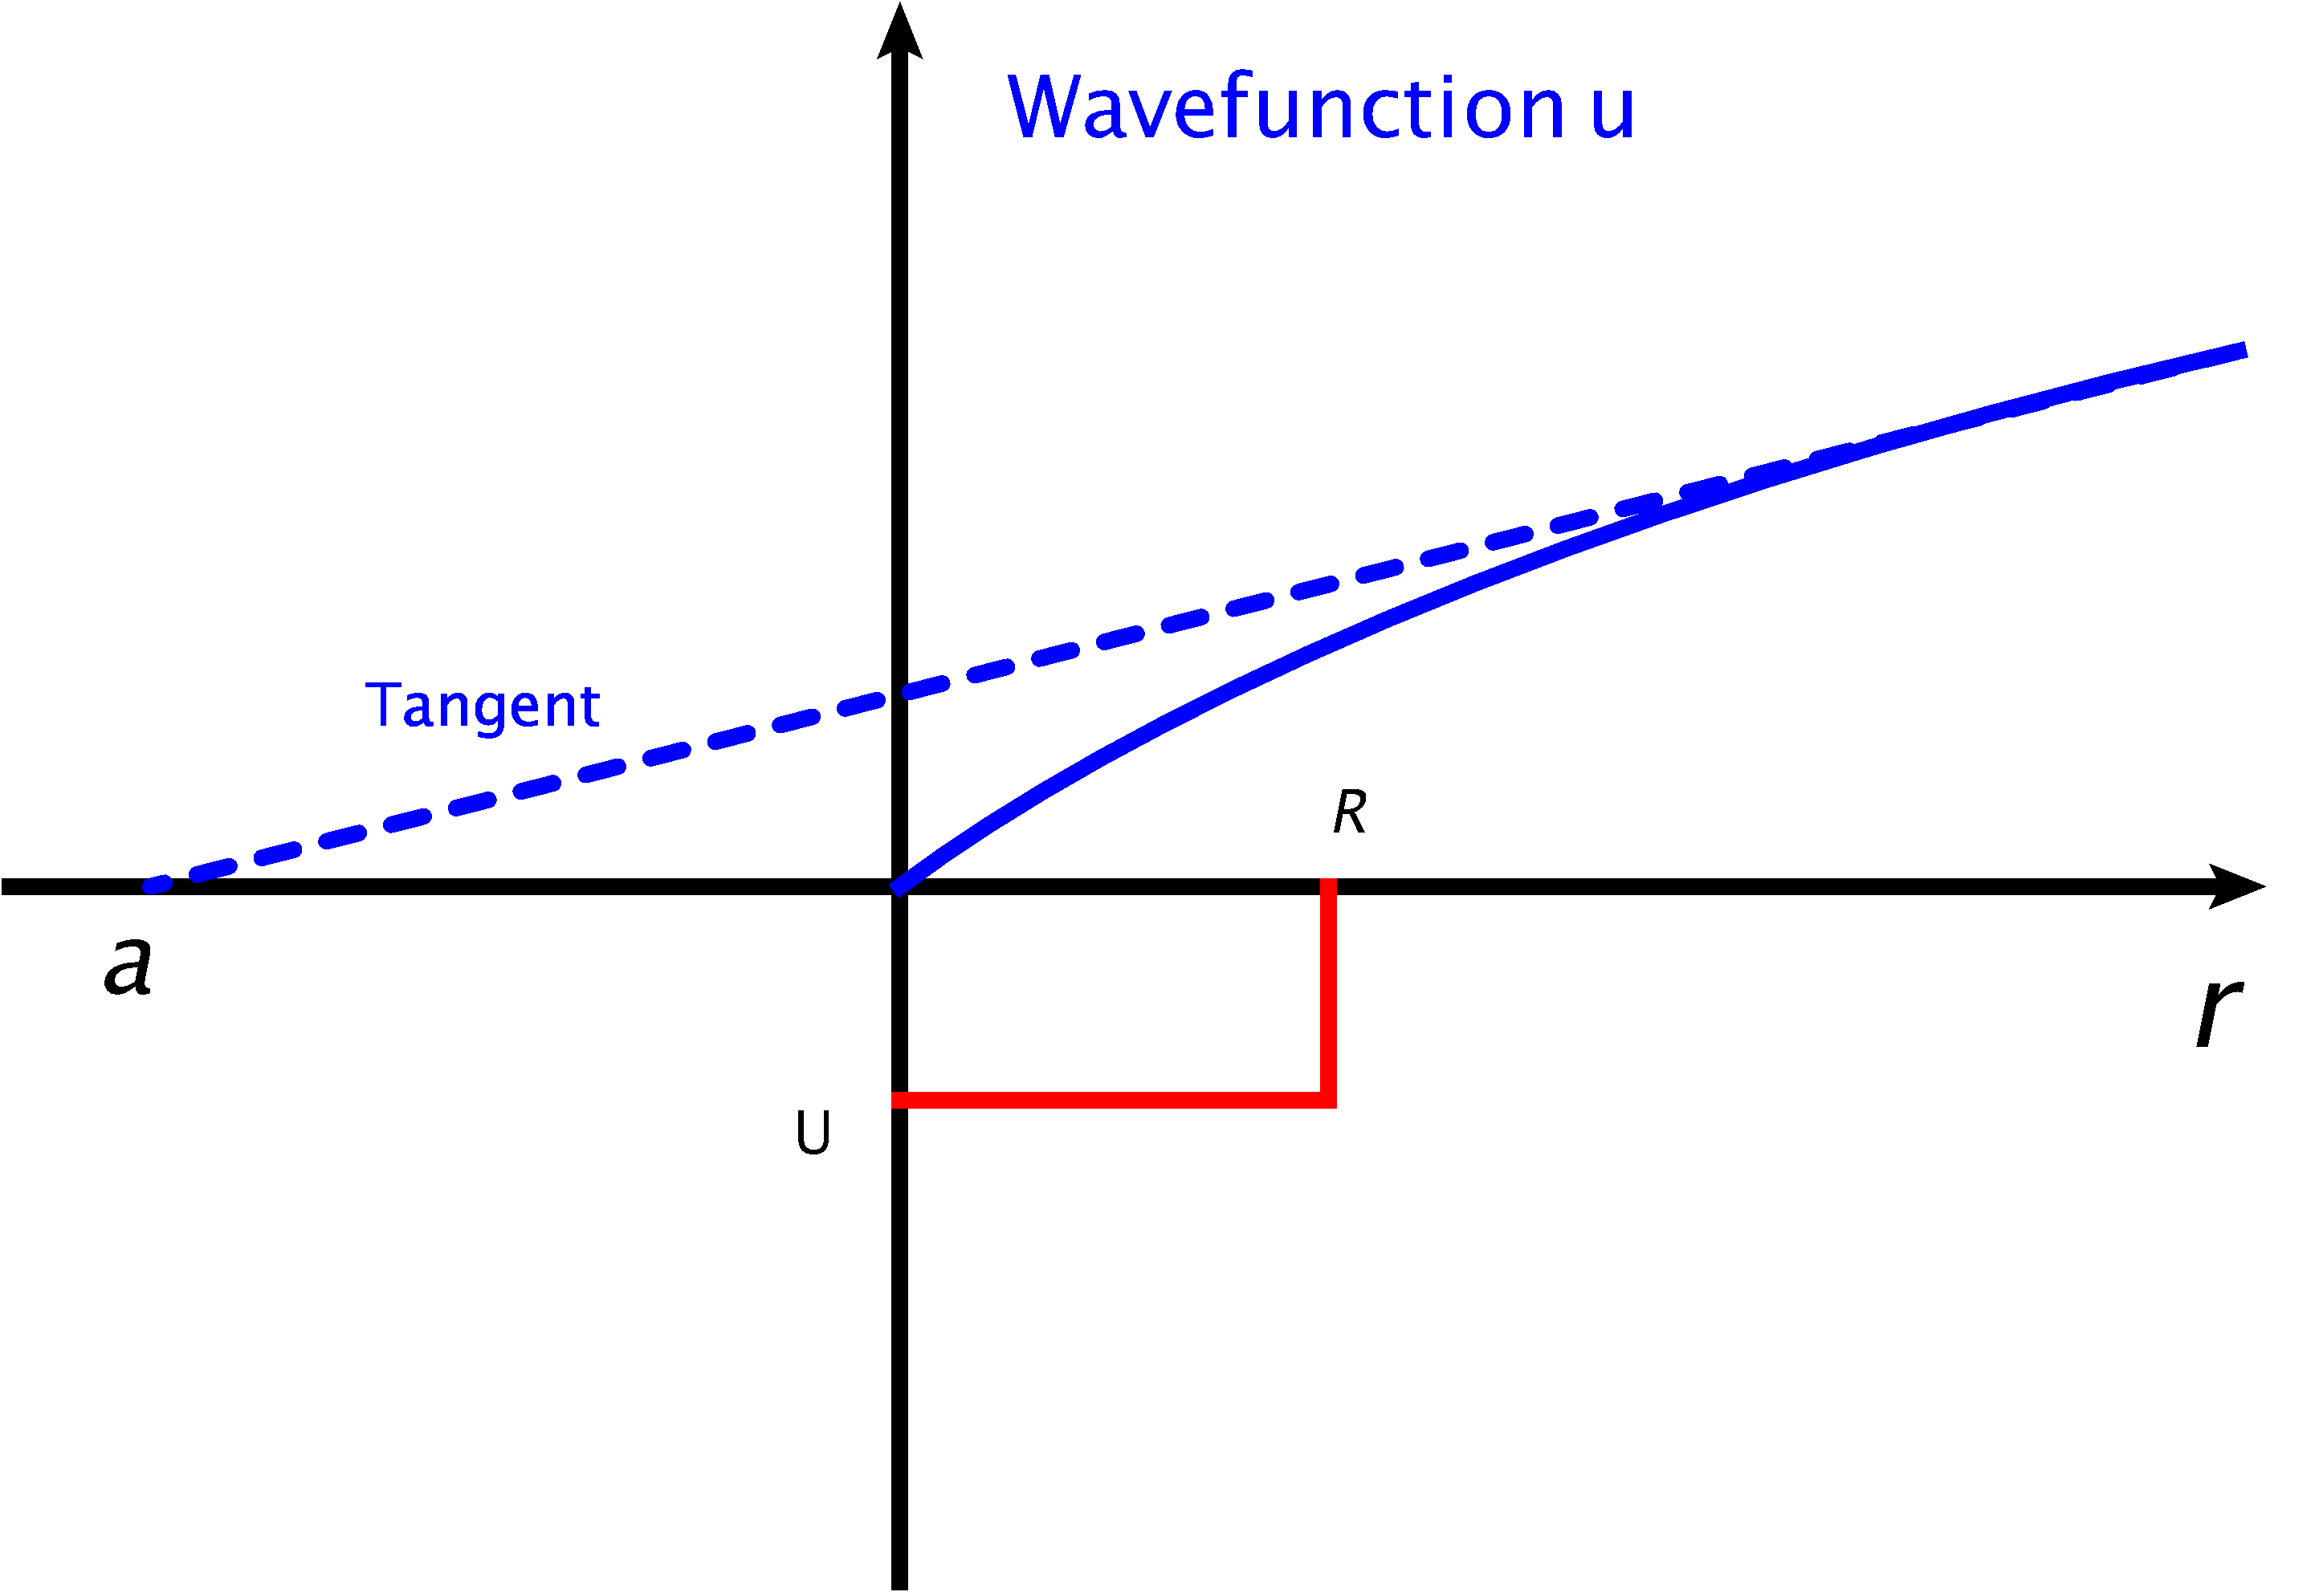
\includegraphics[scale=0.1]{Neg_a.png} 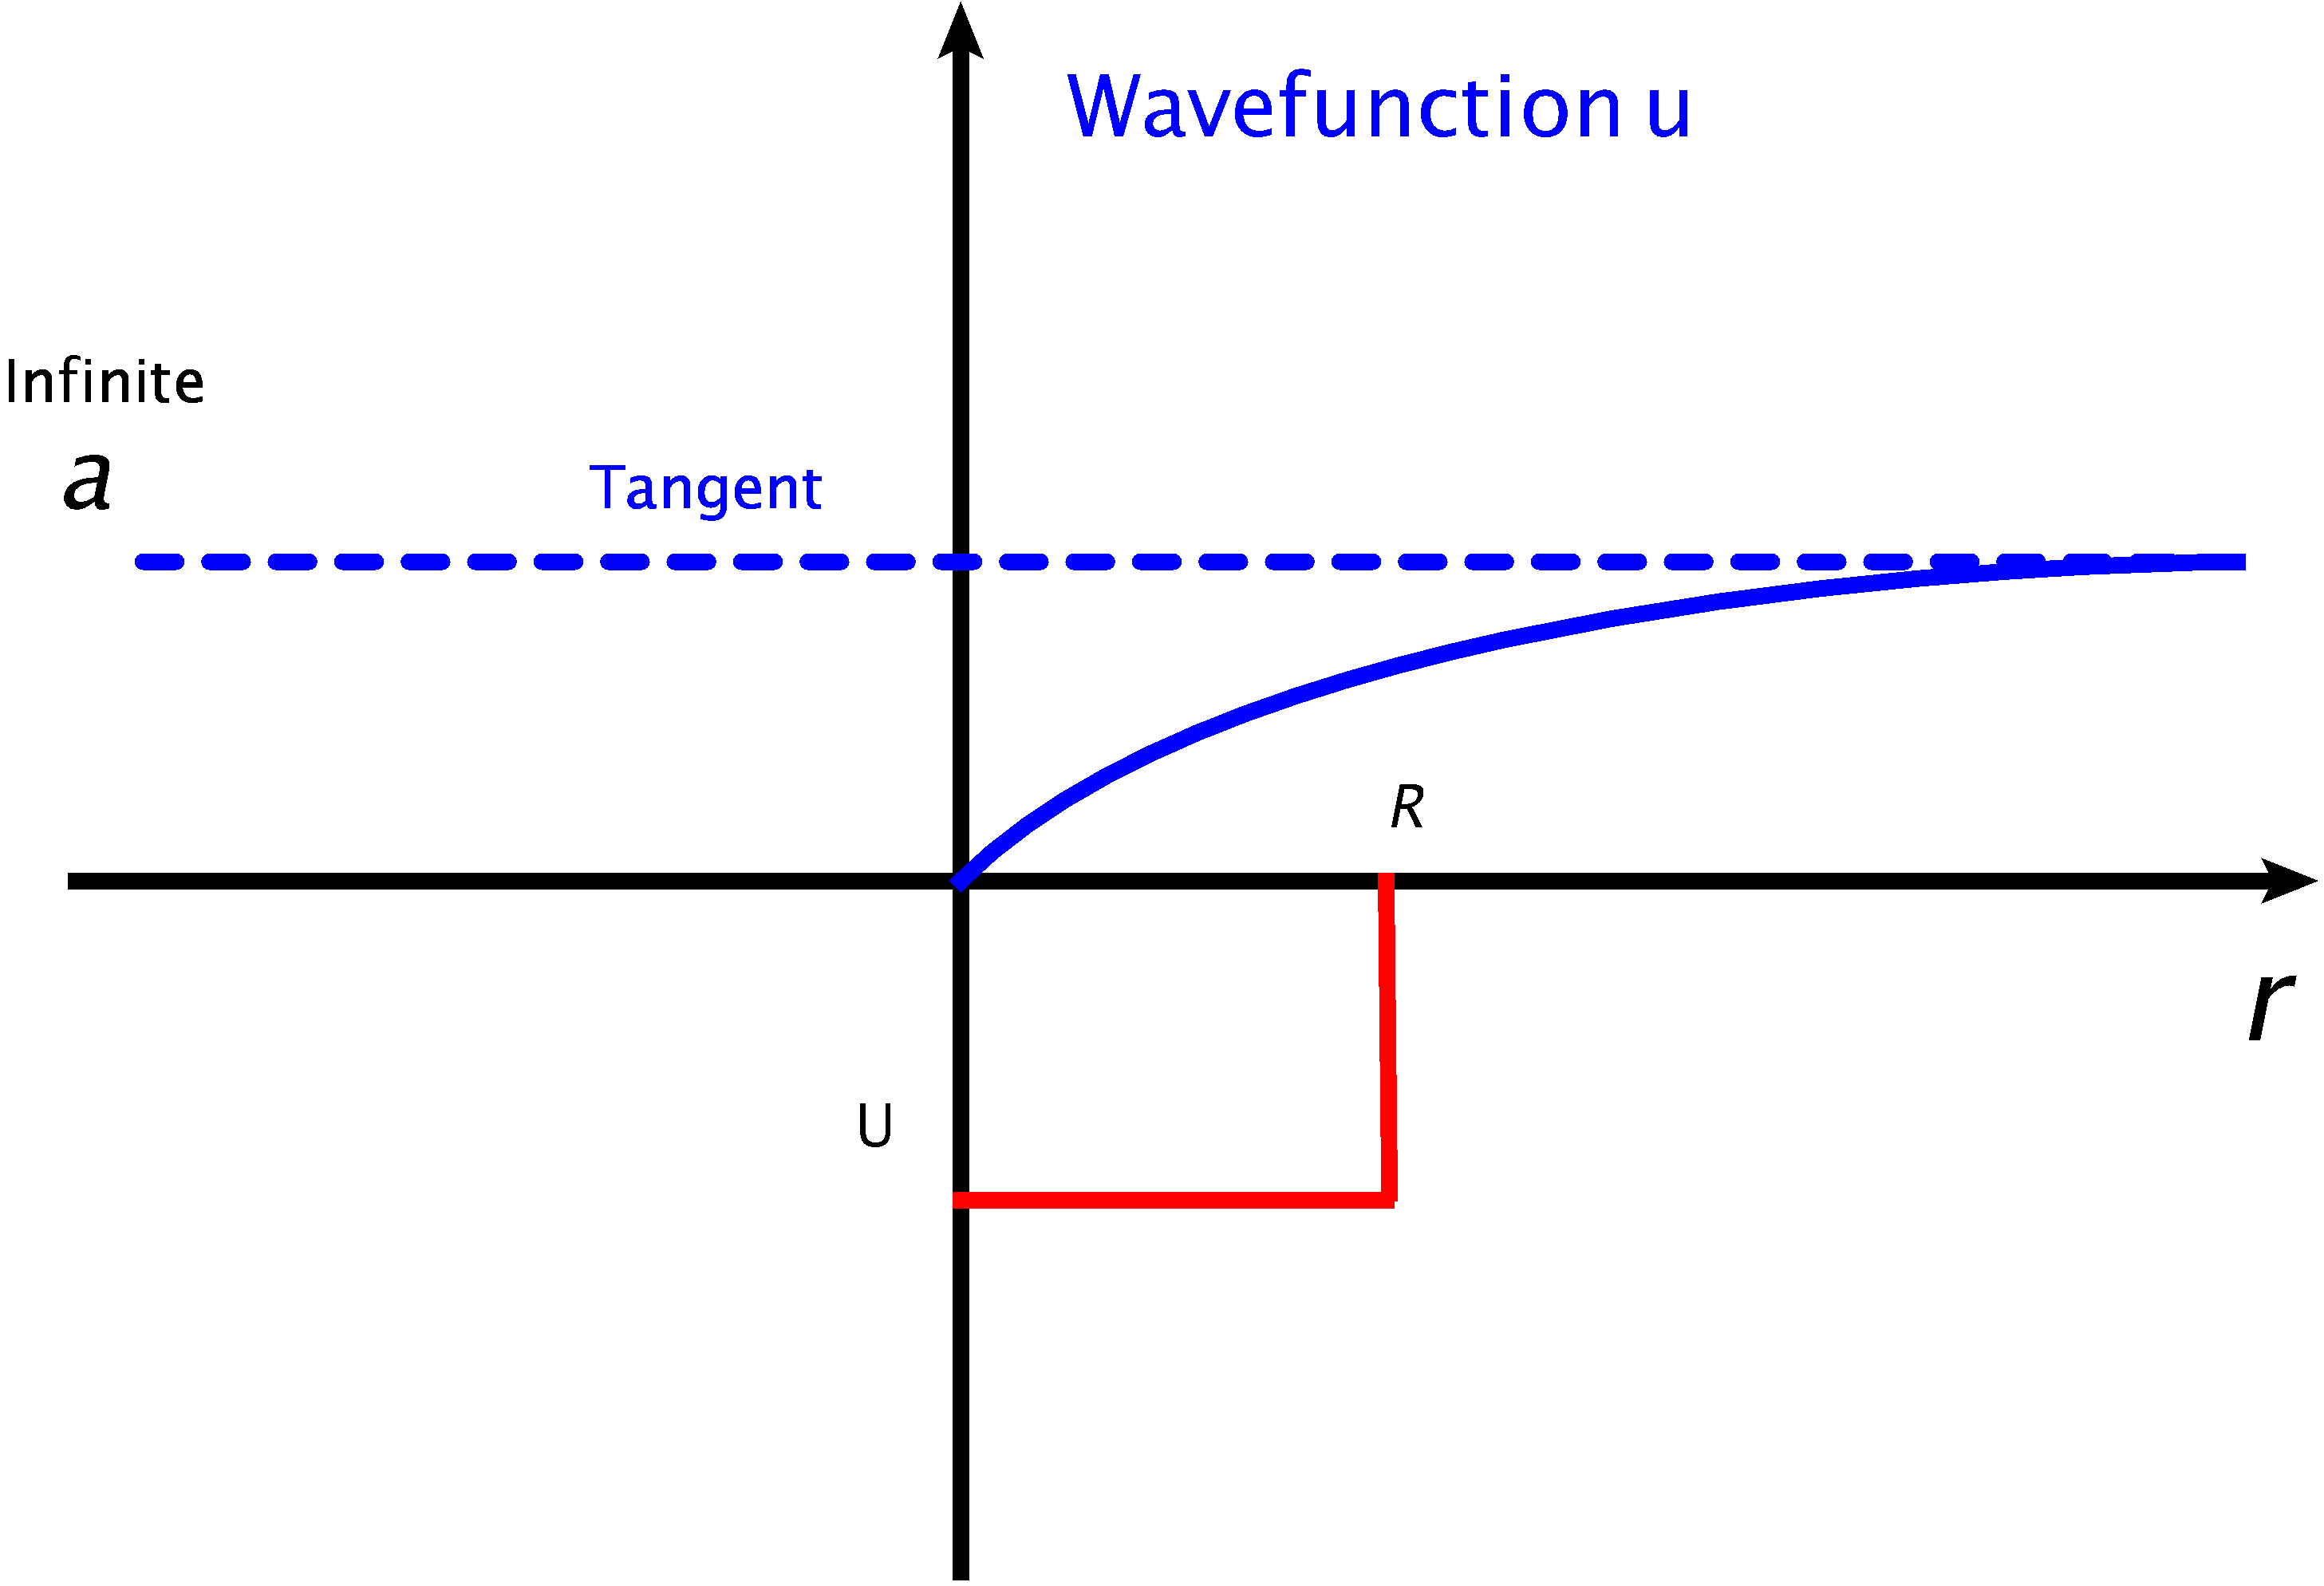
\includegraphics[scale=0.1]{Inf_a.png} 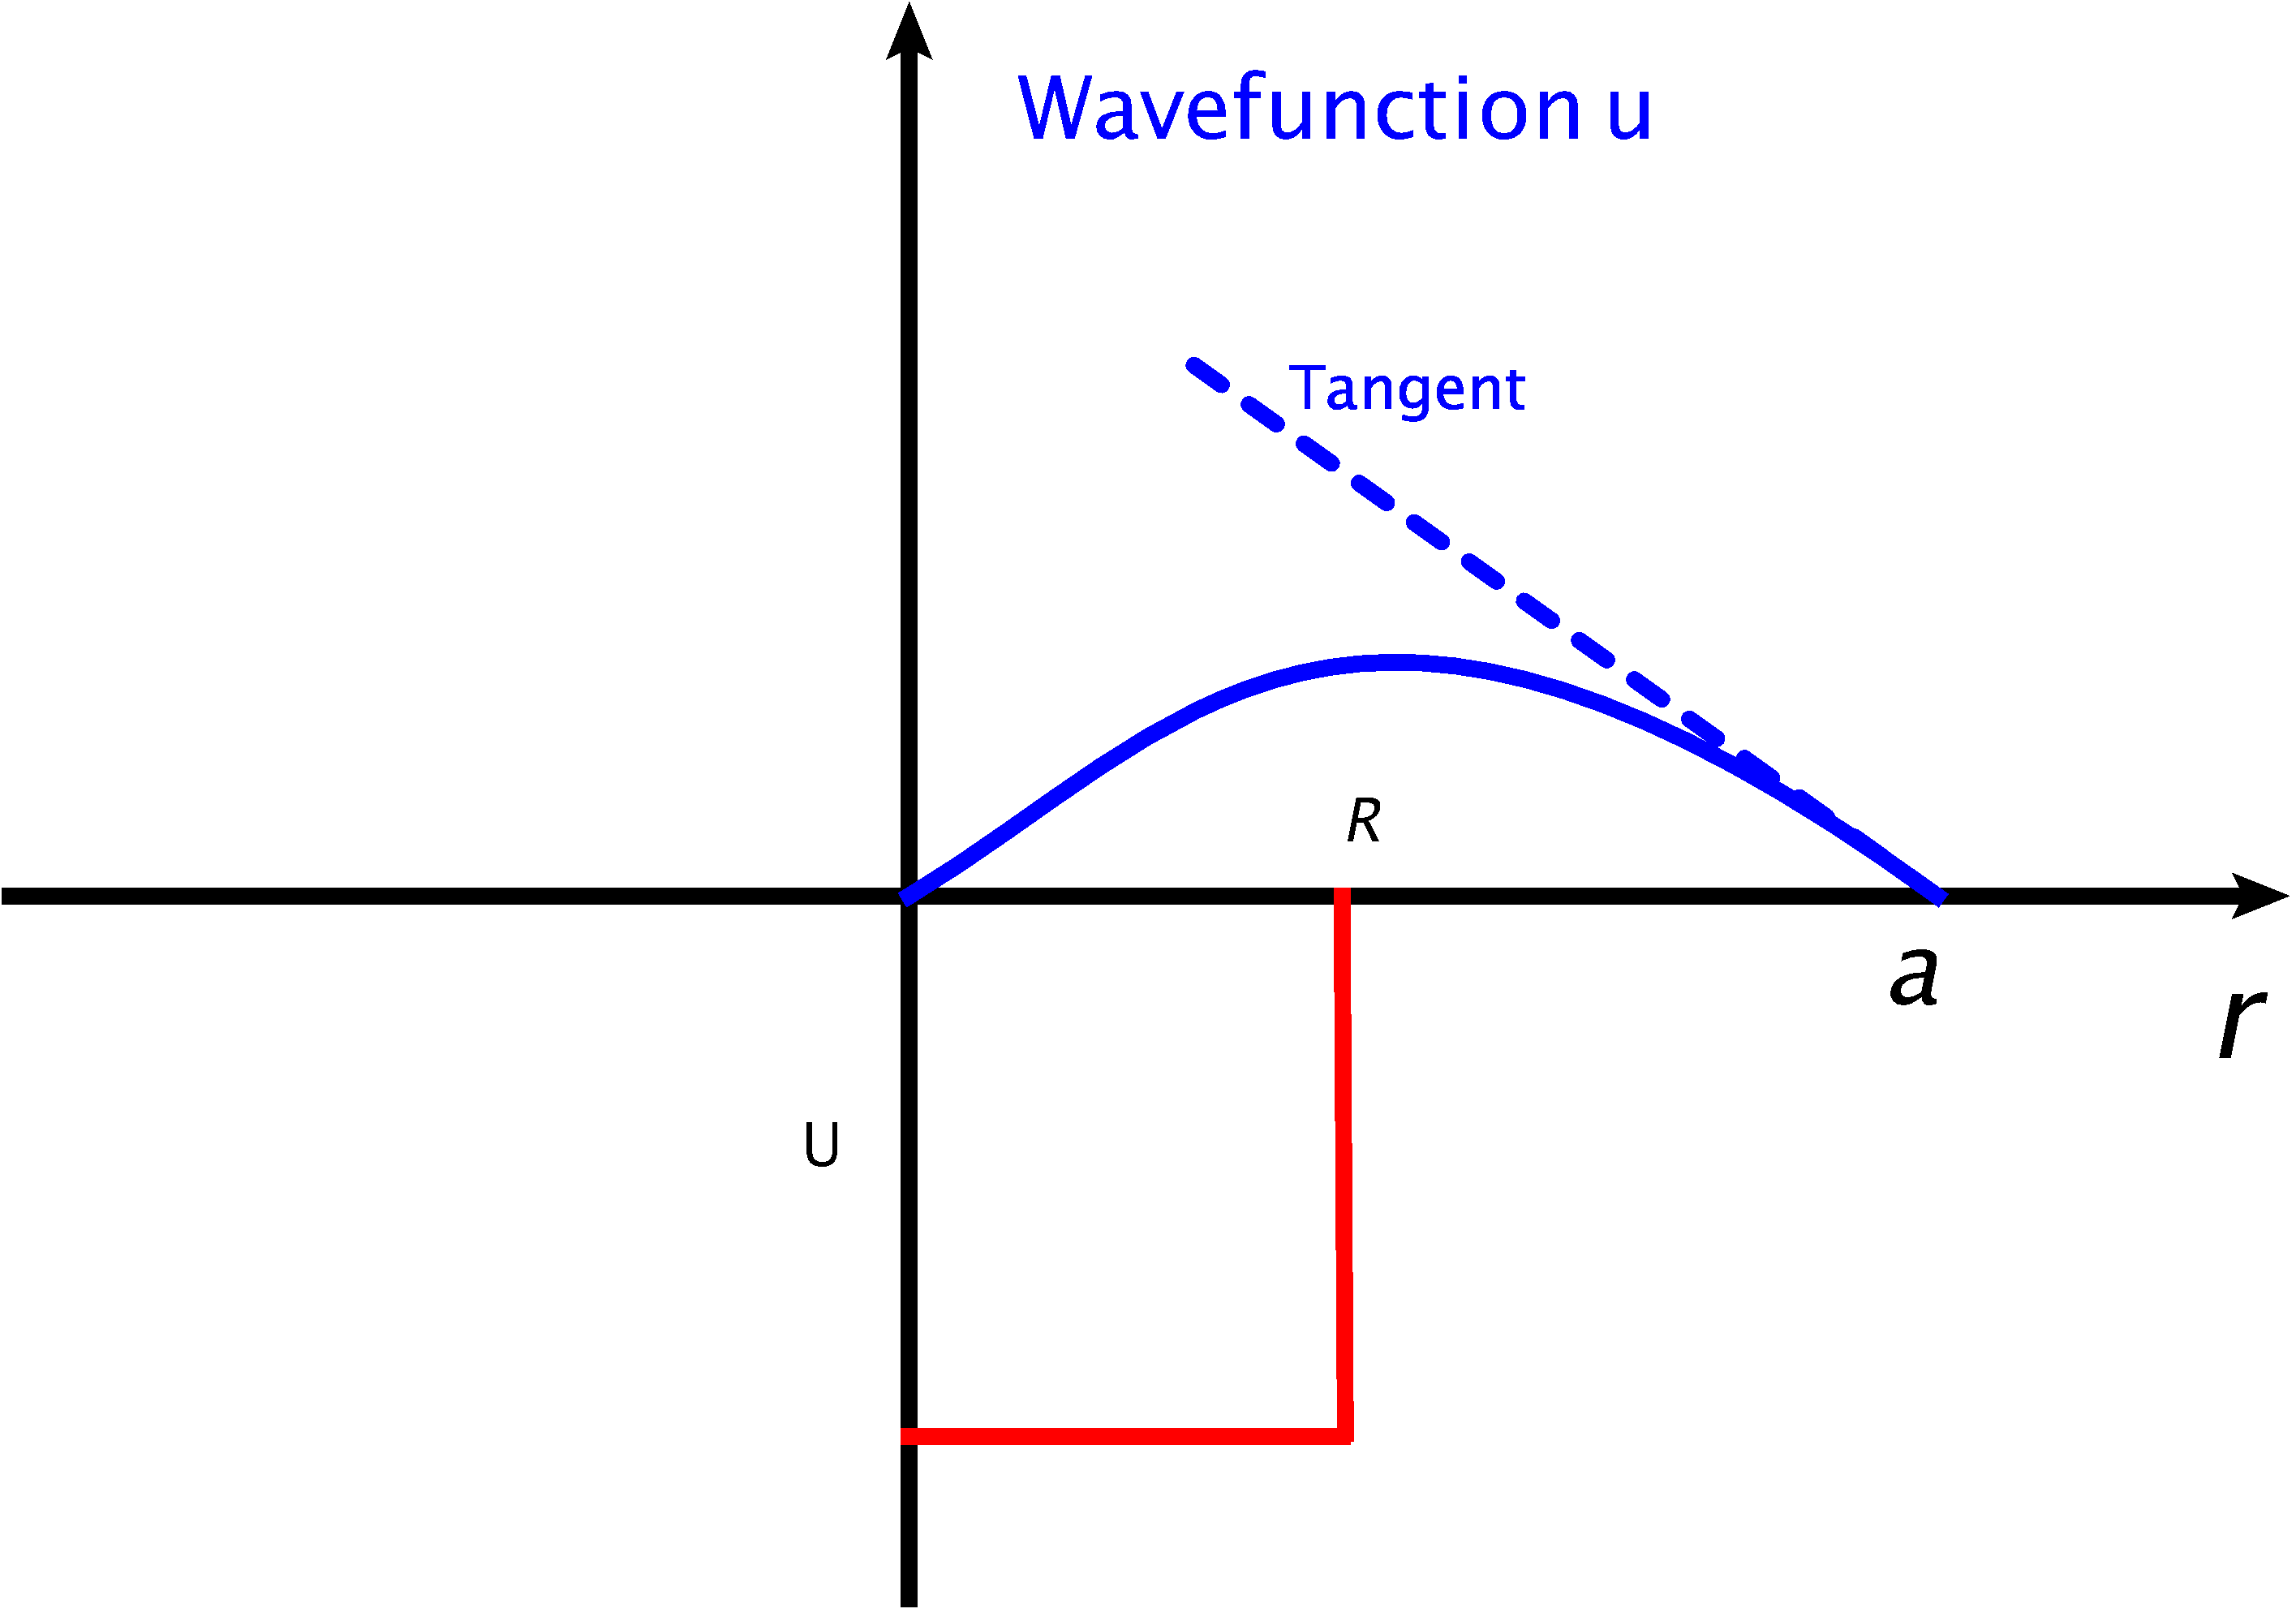
\includegraphics[scale=0.1]{Pos_a.png}
\caption{Scattering Length a) $a_0 < 0$ b) $a_0 = \infty$ and c) $a_0 >0$.}
\end{figure}
This implies that the scattering cross section vanishes when $\tan (KR)/ KR = 1$. \\
Note that the solution for the wavefunction for $r>R$ and in the low energy limit must satisfy
\begin{equation}
\dfrac{d^2 u_0 (r)}{dr^2} =0 \Rightarrow u_0 (r) = D' (r-a_0)
\end{equation}
This is only possible if in the low energy limit $\delta_0 = -k a_0 $. Thus the length scale $a_0$ is the point where the extrapolated wavefunction intersects the x-axis. In other words, it is convenient to define a scattering length such that $u_0 (a_0) =0 $ for $kR<<1$,
\begin{equation}
\begin{split}
u(a_0) &= \sin(k a_0 +\delta_0) = \sin(k a_0) \cos(\delta_0) + \cos(k a_0) \sin(\delta_0) \\
&= \sin(\delta_0) [\sin(k a_0) \cot(\delta_0) + \cos(k a_0) ]\\
&\approx \sin(\delta_0) [k a_0 \cot(\delta_0) + 1 ] \quad \text{low energy limit small } k 
\end{split}
\end{equation}
which implies
\begin{equation}
 a_0  = - \lim_{k \rightarrow 0 } \dfrac{1}{k}\tan(\delta_0) \approx - R \left( \dfrac{\tan (KR)}{KR} -1 \right) \quad \text{where } K=\sqrt{U_0}
\end{equation}
Thus the partial scattering cross section
\begin{equation}
 \sigma_{l=0} = \dfrac{4\pi}{k^2} \dfrac{1}{1+\cot^2(\delta_0)} \approx \dfrac{4\pi}{k^2} \dfrac{(ka_0)^2}{1+(ka_0)^2} \approx 4 \pi a_0^2
\end{equation}

\underline{Limiting Cases:}
\begin{itemize}
\item  $KR << 1$ : $a_0 < 0$ and we have negative scattering length i.e. characteristic of attraction
\item  $KR \rightarrow \pi/2$ : $a_0$ diverges i.e. criterion for a single bound state
\item  $\pi/2< KR < \pi$ : $a_0 > 0$ and we have positive scattering length i.e. characteristic of effective repulsion
\item  $KR \rightarrow \pi$ : $a_0 =0$
\item  $\pi< KR < 3\pi/2$ : $a_0 < 0$ and we have negative scattering length i.e. characteristic of attraction
\item  $KR \rightarrow 3\pi/2$ : $a_0$ diverges i.e. criterion for a second bound state
\item  $3\pi/2< KR < 2\pi$ : $a_0 > 0$ and we have positive scattering length i.e. characteristic of effective repulsion 
\end{itemize}
and so on. \\

When $KR = n\pi$, the scattering cross-section becomes zero and the scattering potential is invisible. This is known as the Ramsauer-Townsend Effect.
\end{document}